%Copyright 2019 Christopher M. Jermaine (cmj4@rice.edu) and Risa B. Myers (rbm2@rice.edu)
%
%Licensed under the Apache License, Version 2.0 (the "License");
%you may not use this file except in compliance with the License.
%You may obtain a copy of the License at
%
%    https://www.apache.org/licenses/LICENSE-2.0
%
%Unless required by applicable law or agreed to in writing, software
%distributed under the License is distributed on an "AS IS" BASIS,
%WITHOUT WARRANTIES OR CONDITIONS OF ANY KIND, either express or implied.
%See the License for the specific language governing permissions and
%limitations under the License.
%===============================================================
\documentclass[aspectratio=169]{beamer}
\mode<presentation> 
{
\usetheme[noshadow, minimal,numbers,riceb,nonav]{Rice}
\usefonttheme[onlymath]{serif}
\setbeamercovered{transparent}
}
\useinnertheme{rectangles}

\usepackage[english]{babel}

\usepackage{amsmath}
\usepackage{mathptmx}
\usepackage{helvet}
\usepackage{courier}
\usepackage[T1]{fontenc}
\usepackage{trajan}
\usepackage{ textcomp }
\renewcommand{\footnotesize}{\tiny}


\usepackage{listings}

\newenvironment{noindentitemize}
{ \begin{itemize}
 \setlength{\itemsep}{1.5ex}
  \setlength{\parsep}{0pt}   
  \setlength{\parskip}{0pt}
 \addtolength{\leftskip}{-2em}
 }
{ \end{itemize} }

\newenvironment{noindentitemize2}
{ \begin{itemize}
  \setlength{\itemsep}{0ex}
  \setlength{\parskip}{0pt}
  \setlength{\parsep}{0pt}   
  \addtolength{\leftskip}{-2em}  }
{ \end{itemize} }

\lstnewenvironment{SQL}
  {\lstset{
        aboveskip=5pt,
        belowskip=5pt,
        escapechar=!,
        mathescape=true,
        upquote=true,
        language=C,
        basicstyle=\linespread{0.94}\ttfamily\normalsize,
        deletekeywords={VALUE, PRIOR},
        showstringspaces=true}
        \vspace{0pt}%
        \noindent\minipage{0.47\textwidth}}
  {\endminipage\vspace{0pt}}
  
\newcommand{\LIKES}{\textrm{LIKES}} 
\newcommand{\FREQUENTS}{\textrm{FREQUENTS}} 
\newcommand{\SERVES}{\textrm{SERVES}} 
\newcommand{\CAFE}{\textrm{CAFE}} 
\newcommand{\COFFEE}{\textrm{COFFEE}} 
\newcommand{\DRINKER}{\textrm{DRINKER}} 
\newcommand{\ALLPEEPS}{\textrm{ALLPEEPS}} 
\newcommand{\ALLCOMBOS}{\textrm{ALLCOMBOS}} 

\setbeamerfont{block body}{size=\tiny}

%===============================================================%

\title[]
{Tools \& Models for Data Science}

\subtitle{Mixture Models}

\author[]{Chris Jermaine \& Risa Myers}
\institute
{
  Rice University 
}

\date[]{}

\subject{Beamer}

\begin{document}

\begin{frame}
 \titlepage
\end{frame}
%***********************************************************
\begin{frame}{Mixture Model Introduction}

\begin{columns}
\begin{column}{0.5\textwidth}
\begin{itemize}
	\item At highest level:
	\begin{itemize}
		\item Have a set of data
		\item And a set of random variables
		\item Don't know which one produced which point
	\end{itemize}
	\item This is a mixture model!
	\item In one line:
	\begin{itemize}
		\item MM: ``hierarchical,'' stochastic, latent variable model
	\end{itemize}
\end{itemize}
\end{column}
\begin{column}{0.5\textwidth}
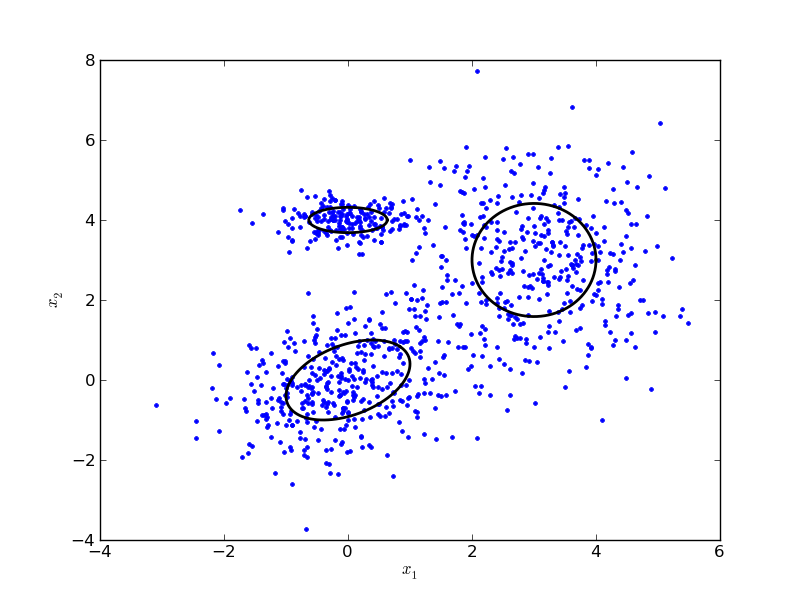
\includegraphics[width=1\textwidth]{lectMM/sample_gmm.png}
\end{column}
\end{columns}

\end{frame}
%***********************************************************
\begin{frame}{Why Use Them?}

\begin{itemize}
	\item Sometimes, we want to segment the data
	\begin{itemize}
		\item Observe a set of test scores
		\item Want 3 types of students: good, average, bad
		\item Associate each with a different Normal distribution
	\end{itemize}
	\item Sometimes, we just want a very flexible model
	\begin{itemize}
		\item A mixture can give a complicated, multi-modal distribution
		\item We can construct these from simple distributions
		\item In reality, not much data is purely normally distributed
	\end{itemize}
\end{itemize}
\end{frame}
%***********************************************************
\begin{frame}{GMM Example}

\begin{columns}
\begin{column}{0.5\textwidth}
\begin{itemize}
	\item Blue curve is what you get if you fit a single normal distribution to the purple data 
	\item Note the shift in the mean
	\item The dashed curves are the mixture distributions
	\item Note there are actually 3 normal distributions in this plot
\end{itemize}
\end{column}
\begin{column}{0.5\textwidth}
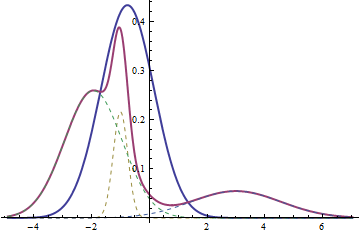
\includegraphics[width=0.8\textwidth]{lectMM/W2PQO.png}
\end{column}
\end{columns}
\end{frame}
%***********************************************************
\begin{frame}{Mixture Model Introduction}

\begin{itemize}
	\item Choose the parameters for each normal distribution
	\item And a weighting for each mixture
	\item Use these to produce a set of data $x_1, x_2, ..., x_n$
        \begin{itemize}
		\item And a set of hidden (latent) indicators $c_1, c_2, ..., c_n$ specifying which mixture was selected
	\end{itemize}
	\item MM begins with a distribution function $f$
       	\begin{itemize}
		\item Common $f$: Gaussian, Multinomial, Gamma, etc.
		\item We have $k$ sets of parameters for $f$: $\theta_1, \theta_2, ..., \theta_k$
		\item And a probability vector $\pi$ that tells us how important each mixture component is	
		\item Note: we can have a mixture model where each component is from a different distribution
		\item This is uncommon, though
	\end{itemize}
\end{itemize}
\end{frame}

%***********************************************************
\begin{frame}[fragile]{Mixture Model Introduction}
\begin{itemize}
	\item Pseudo-code to produce $n$ observations is:
\end{itemize}
\begin{SQL}
for i = 1 to n do:
  $c_i \sim \textrm{Categorical}(\pi)$
  $x_i \sim f(\theta_{c_i})$
\end{SQL} 
\end{frame}
%***********************************************************
\begin{frame}{Mixture Model PDF}

\begin{itemize}
\item In general, PDF is:
$$P(x_1, x_2, ..., x_n) = \prod_i^n \left( \sum_j^K \pi_j f (x_i | \theta_j) \right)$$
\item Where $n$ is the number of data points
\item Where $K$ is the number of mixtures
\item Where $f$ is the PDF for distribution $k$
\item[?] Why?
\end{itemize}
\end{frame}
%***********************************************************
\begin{frame}{Mixture Model PDF}

\begin{itemize}
\item In general, PDF is:
$$P(x_1, x_2, ..., x_n) = \prod_i^n \left( \sum_j^K \pi_j f (x_i | \theta_j) \right)$$
\item Why?
\begin{itemize}
 \item Likelihood of choosing component $j$, then $j$ producing $x$ is:
			$$\pi_j f (x | \theta_j) $$
		\item Since $n$ data points are independent, we have a product over the likelihoods\end{itemize}
\end{itemize}
\end{frame}
%***********************************************************
\begin{frame}{Mixture Model PDF}

\begin{itemize}
\item For each data point, the PDF is:
% Pr(x) = 
$$ \sum_j^k \pi_j f (x_i | \theta_j)$$
\item We can represent  the choice, $c$  as a 1-of-k valued vector, where one dimension is 1 and the rest are all 0
\item The dimension is set to 1 if that mixture model generated the data point
\item and set to 0 otherwise
\item It follows that $p(c_j = 1 ) = \pi_j$
\item and that $\sum_j^k \pi_j = 1$
\item To get the marginal distribution of $x$ we sum the joint distribution over all possible states of $c$
\end{itemize}
\end{frame}
%***********************************************************
\begin{frame}{Learning}

\begin{itemize}
	\item Would be easy if we knew $c_1, c_2, ..., c_n$
	\item Where $c_j$ is the indicator of which mixture distribution produced data point $j$
	\begin{itemize}
		\item In that case, we'd have $k$ different MLE problems
%		$$ Log\ p(X | \pi, \theta) = \sum_1^n log \Big(\sum_j^k \pi_j f (x_i | \theta_j)\Big)$$
\item That is, to learn, partition the data points according to $c$ values
		\item Then perform an MLE separately on each
 		\item For standard distributions, this is easy
 		\item Example, for 1-D Normal
\begin{itemize}
		\item MLE for $\mu_j$ is mean of points with $c_i = j$
 		\item MLE for $\sigma_j$ is std. dev. of points with $c_i = j$
	\end{itemize}
	\end{itemize}
	\item But there are complications in doing this
	% Bishop book Chapter 9
	% there are K! ways of assigning K parameters to K components
	% plus singularity issues if x = \mu_k
	\item And we don't know the $c_j$ values anyway!
\end{itemize}

\end{frame}
%***********************************************************
\begin{frame}{Learning}

\begin{itemize}
	\item But we don't!
	\item Standard methods:
	\begin{itemize}
	\item MCMC (sample $c_1, c_2, ..., c_n$): Stochastic, Bayesian approach, not covered in this course
	\item EM
	\end{itemize}
\end{itemize}

\end{frame}
%***********************************************************
\begin{frame}{EM for Mixture Models...}

\begin{itemize}
\item The Patriarch: The Gaussian Mixture Model (GMM)
$$P(x_1, x_2, ..., x_n) = \prod_i \left( \sum_j \pi_j \textrm{Normal} (x_i | \mu_j, \sigma^2_j) \right)$$
\end{itemize}
\begin{enumerate}
\item Make non-stupid guesses for the means, variances, and the mixing parameters
\item E-step: Use the current parameter values to asign each data point to the most likely  mixture component
\item M-step: Use the expected values to update the mixture parameters
\end{enumerate}
\end{frame}
%***********************************************************
\begin{frame}{Example GMM}

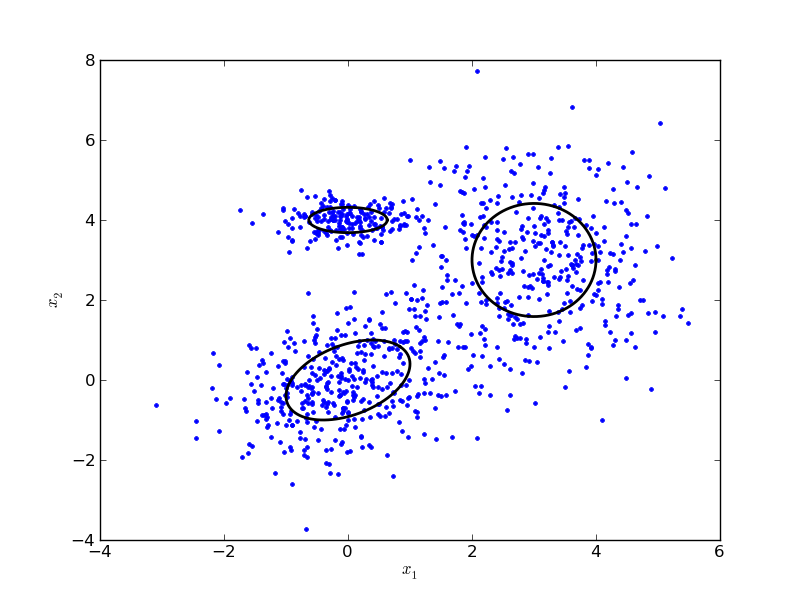
\includegraphics[width=0.7\textwidth]{lectMM/sample_gmm.png}
\end{frame}
%***********************************************************
\begin{frame}{Mixture of Dirichlets}

\begin{itemize}
\item Imagine that I have a large corpus of text documents
\item And I want to understand the various types of documents present
\item Basically, I want to cluster the documents
\item We might view the TF (term frequency) vector as being produced as a sample from a Dirichlet distribution
\item[?] What's a Dirichlet distribution?
\end{itemize}
\end{frame}
%%***********************************************************
%\begin{frame}{Beta Distribution}
%\begin{columns}
%\begin{column}{0.5\textwidth}
%\begin{itemize}
%\item \textcolor{red}{Generalization of Beta distribution to many dimensions}\\
%
%\item What is the Beta distribution?
%	\begin{itemize}
%	\item Continuous distribution
%	\item Returns a value in [0,1]
%	\item Has two parameters: $\alpha$ and $\beta$, that control the shape
%	\item Used for RVs in a finite range
%	\item Can be represented as a ratio of Gamma distributions
%	\end{itemize}
%\end{itemize}
%\end{column}
%\begin{column}{0.5\textwidth}
%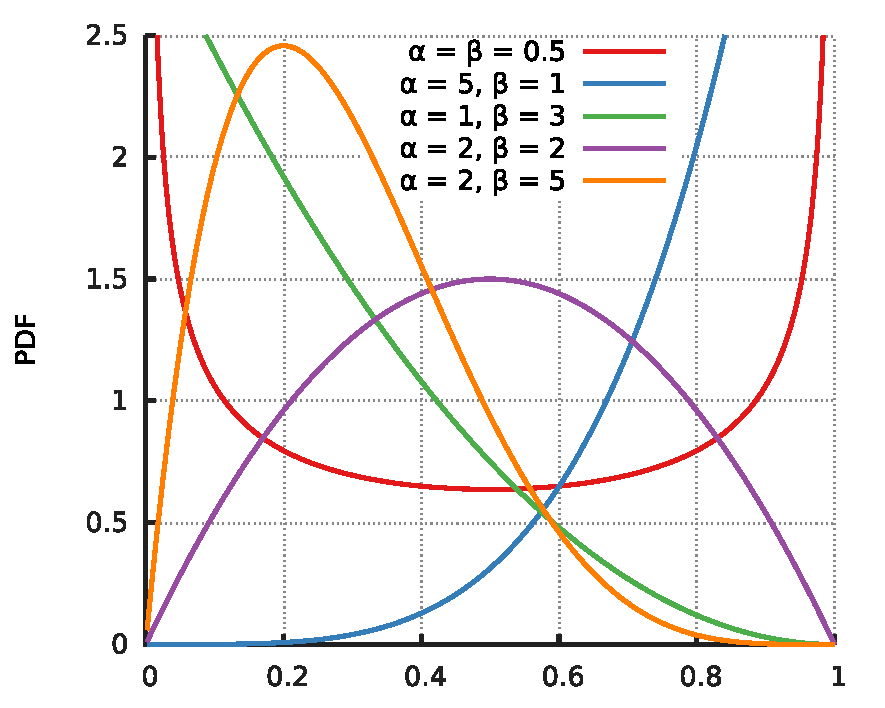
\includegraphics[width=1\textwidth]{lectMM/Beta_distribution_pdf.pdf}
%\end{column}
%\end{columns}
%\end{frame}
%%***********************************************************
%\begin{frame}{Gamma Distribution}
%\begin{columns}
%\begin{column}{0.5\textwidth}
%\begin{itemize}
%\item What is the Gamma distribution?
%	\begin{itemize}
%	\item Continuous distribution
%	\item Has two parameters: shape: $a$ and scale:$1/\theta$
%	\item Parameters must be positive real numbers
%	\item Used to model time to failure or waiting times
%	\end{itemize}
%\end{itemize}
%\end{column}
%\begin{column}{0.5\textwidth}
%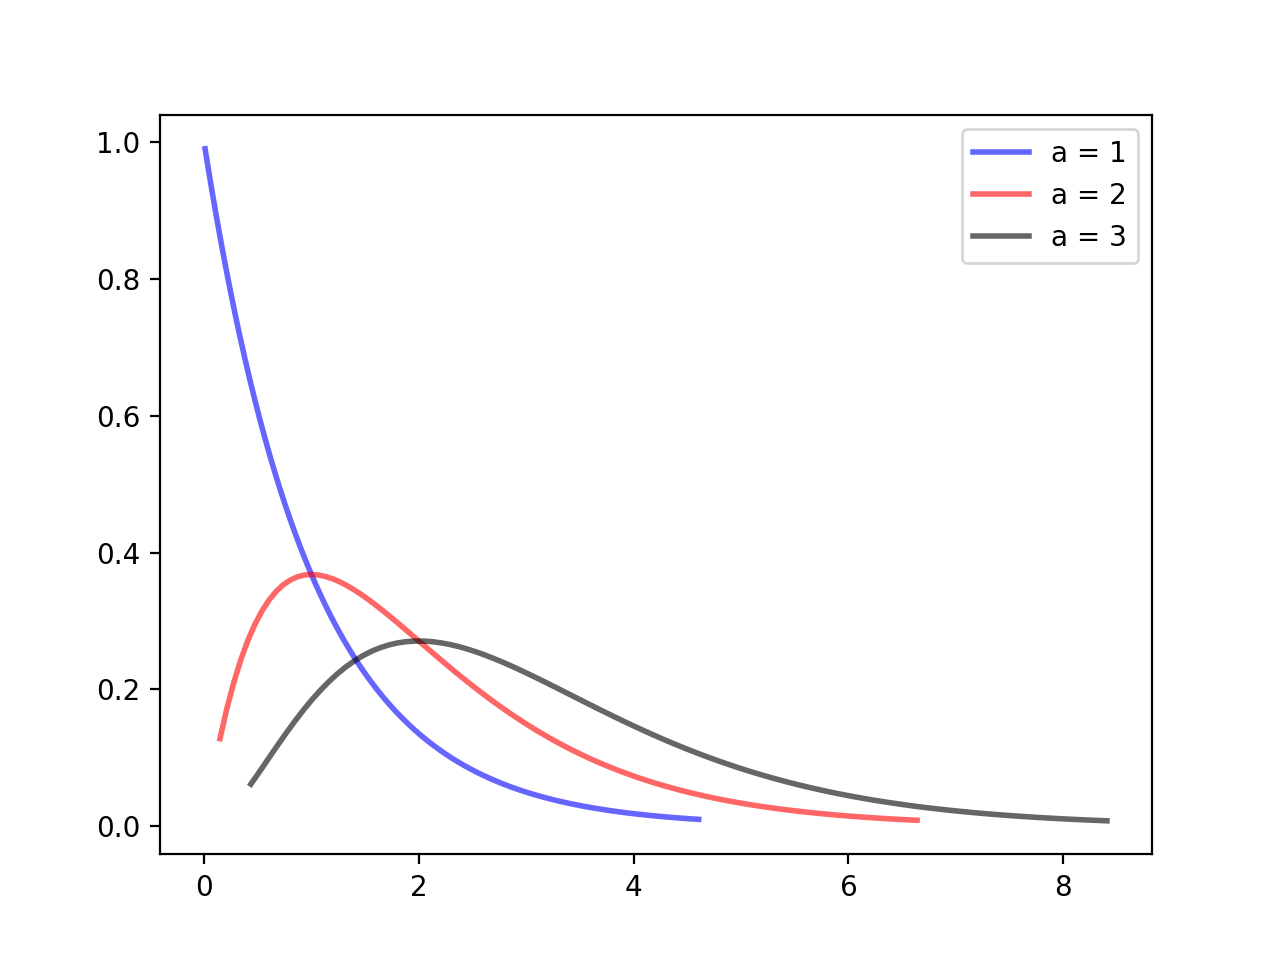
\includegraphics[width=1\textwidth]{lectMM/gamma.png}
%\end{column}
%\end{columns}
%\end{frame}
%%***********************************************************
%\begin{frame}{Dirichlet Distribution}
%\begin{itemize}
%\item Generalization of Beta distribution to many dimensions
%	\begin{itemize}
%	\item Takes params $v_1, v_2, ..., v_m$
%	\item Produces $m$ values that sum to 1
%	\item To generate, sample from $m$ Gammas, each with shape $v_j$
%	\item $i$th value is $i$th Gamma's fractional contribution to total
%	\item Expected value of $i$th is $v_j / \sum_{j'} v_{j'}$
%	\end{itemize}
%\end{itemize}
%\end{frame}
%***********************************************************
\begin{frame}{Dirichlet Distribution}
\begin{itemize}
\item Generalization of Beta to many dimensions
\item Produces vectors on the ``simplex''
	\begin{itemize}
	\item That is, vectors whose entries sum to 1
	\item Hence, \color{red}{used as a distribution to produce vectors of probabilities}
	\end{itemize}
\item Takes params $\langle v_1, v_2, ..., v_m \rangle$
	\begin{itemize}
	\item Produces $m$ values that sum to 1
	\item ``looks'' like a probability vector
	\item To generate, sample from $m$ Gammas, each with shape $v_j$
	\item $i$th value is $i$th Gamma's fractional contribution to total
	\end{itemize}
\end{itemize}
\end{frame}
%***********************************************************
\begin{frame}{Dirichlet Distribution}
\begin{itemize}
	\item Expected value of $i$th is $\frac{v_j}{\sum_{j'} v_{j'}}$
	\begin{itemize}
	\item Then what's the difference between parameter vector $\langle 1, 2, 3 \rangle$
	and $\langle 10, 20, 30 \rangle$?
	\end{itemize}
	\item Both result in Dirichlets with same mean
	\begin{itemize}
	\item But smaller parameters allow more variance
	\item So the former has much more variance... resulting Dirichlet could produce $\langle 0.2, 0.1, 0.7 \rangle$
	\item Latter will always produce something like $\langle 0.1666, 0.3333, 0.5 \rangle$
	\item If we normalize the parameter vectors (divide by their sum) we get 
	\item[] $6 \times \langle 0.166, 0.333, 0.5 \rangle$ and
	\item[] $60 \times \langle 0.166, 0.333, 0.5 \rangle$
	\item The higher the normalization constant is, the closer the samples will be to the mean
	\end{itemize}
\end{itemize}
	\end{frame}
%***********************************************************
\begin{frame}{Dirichlet Distribution}

\begin{columns}
\begin{column}{0.5\textwidth}
\begin{enumerate}
\item $\langle 1,1,1 \rangle$ Everything is equally likely
\item  $\langle 2,2,2 \rangle$ As the parameters grow, on expectation, the samples are more concentrated
\item $\langle 10,10,10 \rangle$ As the numbers continue to get bigger, the samples are more likely to be $\frac{1}{3},\frac{1}{3},\frac{1}{3}$
\item $\langle 2,10,2 \rangle$ If a parameter is larger, that dimension get more weight
\item $\langle 2,2,10 \rangle$
\item $\langle 0.9,0.9,0.9 \rangle$ When parameters are < 1, the samples go to the outside (more extreme differences)
\end{enumerate}
\end{column}
\begin{column}{0.5\textwidth}
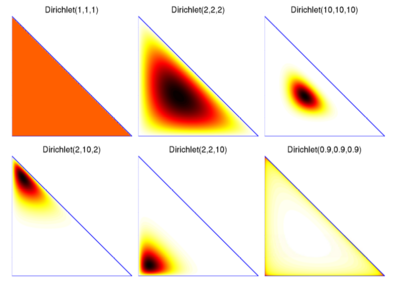
\includegraphics[width=1\textwidth]{lectMM/400px-Dirichlet.png}\footnote{\url{www.cs.cmu.edu/~epxing/Class/10701-08s/recitation/dirichlet.pdf}}
\end{column}
\end{columns}
\end{frame}

%***********************************************************
\begin{frame}{Mixture of Dirichlets Application}

\begin{itemize}
\item Imagine that I have a large corpus of text documents
\item And I want to understand the various types of documents present
\item Basically, I want to cluster the documents
\item We might view the TF (term frequency) vector as being produced as a sample from a Dirichlet distribution
\item TF vector is basically a vector of probabilities
\end{itemize}
\end{frame}


%***********************************************************
\begin{frame}{Mixture of Dirichlets Example}

\begin{itemize}
\item If param vector for $j$th Dirichlet is $\alpha_j$, then PDF is:
$$P(x_1, x_2, ..., x_n) = \prod_i \left( \sum_j \pi_j \textrm{Dirichlet} (x_i | \alpha_j) \right)$$
%\item Example:
%	\begin{itemize}
	\item Take all the papers Chris has written, all the papers Luay has written
	\item Dictionary has words: $\langle$ biology, databases, phylogenetics, statistics $\rangle$
	\item Might get $\alpha_{\textrm{Chris}} = \langle .5, 12, 1.2, 8 \rangle$
	\item Means Chris' mean probability vector is $\langle \frac{.5}{21.7},  \frac{12}{21.7},  \frac{1,2}{21.7}  \frac{8}{21.7} \rangle = \langle 0.02, 0.55, 0.055, 0.37 \rangle$	
	\item For most docs, Chris is most likely to write the word ``databases''
	\item Might get $\alpha_{\textrm{Luay}} = \langle 11, 2, 18, 3.2 \rangle$
	\item His mean probability vector is $\langle 0.32, 0.06, 0.53, 0.09 \rangle$	
	\item Means for most docs, he's most likely to write the word ``phylogenetics''
%\end{itemize}
\item So, we have learned how likely each topic is to appear in each author's publications
\end{itemize}
\end{frame}
%***********************************************************

\begin{frame}{Mixture of Experts}

\begin{columns}
\begin{column}{0.5\textwidth}
\begin{itemize}
\item Used for regression/classification
\item Uses a combination of simpler models to form a better model
\item Each simpler model covers a range of input values
\item We have a switch that determines which model is in place
\end{itemize}
\end{column}
\begin{column}{0.5\textwidth}
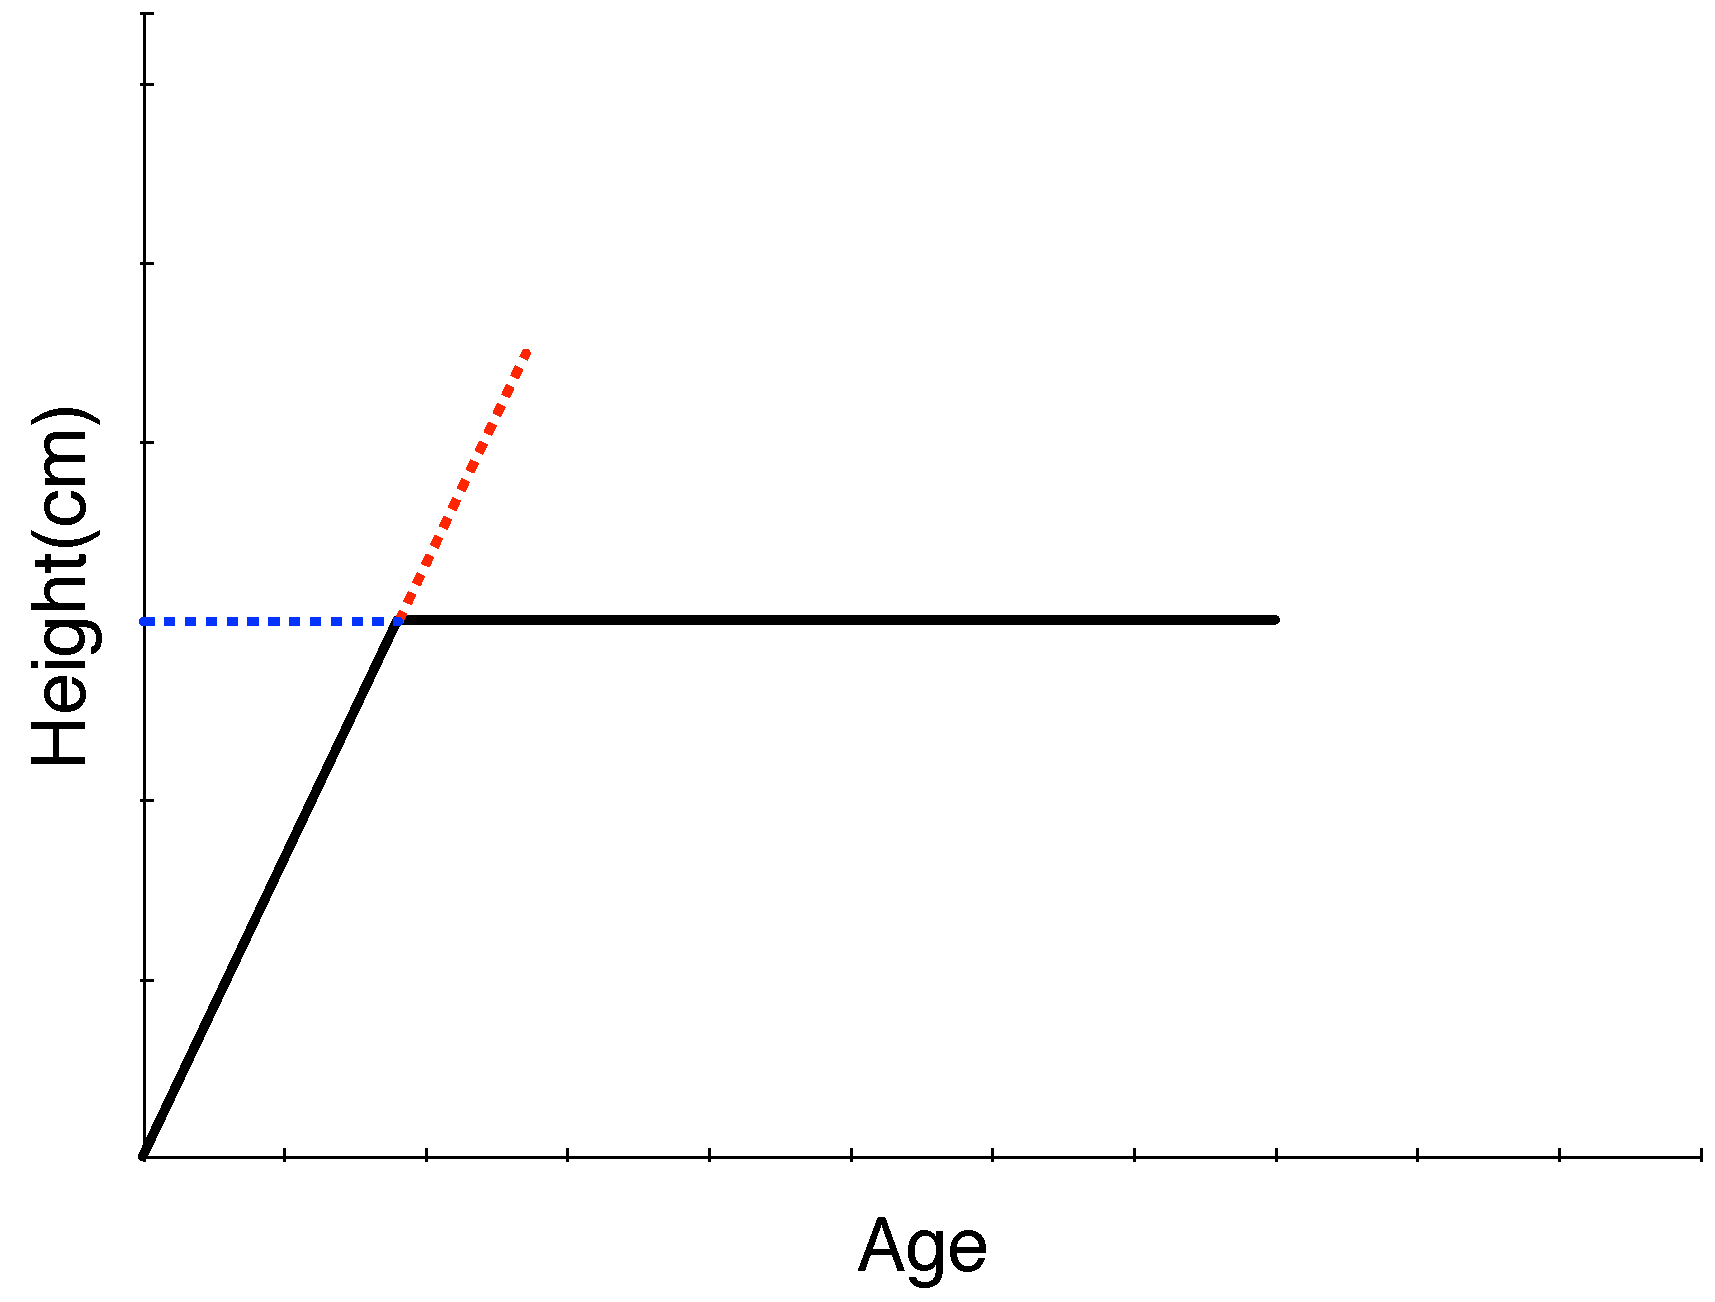
\includegraphics[width=1\textwidth]{lectMM/ageVsHeightV1.pdf}
\end{column}
\end{columns}
\end{frame}
%***********************************************************

\begin{frame}{Mixture of Experts}

\begin{itemize}
	\item In ``classical'' GLMs
	\item Use dot product $x \cdot r = \sum_j x_j \times r_j$ to get ``natural'' parameter for error distribution
	\item Ex: Normal (least squares) regression:
	$$f (y | x) = \textrm{Normal} (y | x \cdot r, \sigma^2)$$
\end{itemize}
\end{frame}
%***********************************************************

\begin{frame}{Mixture of Experts}

\begin{itemize}
	\item In ``classical'' GLMs
	\item Use dot product $x \cdot r = \sum_j x_j \times r_j$ to get ``natural'' parameter for error dist
	\item Ex: Normal (least squares) regression:
	$$f (y | x) = \textrm{Normal} (y | x \cdot r, \sigma^2)$$
\item Now, let's have a mixture of these
\begin{itemize}
	\item Instead of $r$, we have $r_1, r_2, ..., r_k$
	\item Instead of $\sigma^2$, we have $\sigma^2_1, \sigma^2_2, ..., \sigma^2_k$
\end{itemize}
\end{itemize}
\end{frame}
%***********************************************************

\begin{frame}{Mixture of Experts}

\begin{itemize}
\item Mixture proportions computed by looking at $x$
	\begin{itemize}
	\item Each component has a gating vector $\eta$
\item We use a ``softmax gating network'' to get $\pi$ for a given $x$... that is:
	$$\pi_j = \frac{\exp (x \cdot \eta_j)}{\sum_{j'} \exp (x \cdot \eta_{j'})}$$
	\end{itemize}
\item In other words, we normalize the mixture selections to sum to 1
\end{itemize}
\end{frame}

%%***********************************************************
%
%\begin{frame}{Softmax}
%
%\begin{itemize}
%\item 
%\end{itemize}
%\end{frame}
%


%%***********************************************************
%
%\begin{frame}{Mixture of Experts Motivation}
%
%\begin{itemize}
%	\item Use dot product $x \cdot r = \sum_j x_j \times r_j$ to get ``natural'' parameter for error dist
%	\item Ex: Normal (least squares) regression:
%	$$f (y | x) = \textrm{Normal} (y | x \cdot r, \sigma^2)$$
%\end{itemize}
%\end{frame}
%***********************************************************
%***********************************************************

\begin{frame}{Mixture of Experts}

\begin{itemize}
\item If param vector for $j$th Dirichlet is $\alpha_j$, then PDF is:
$$P(x_1, x_2, ..., x_n) = \prod_i \left( \sum_j \pi_j \textrm{Dirichlet} (x_i | \alpha_j) \right)$$
\item So PDF is:
$$P(x_1, x_2, ..., x_n) = \prod_i \left( \sum_j \frac{\exp (x_i \cdot \eta_j)}{\sum_j' \exp (x_i \cdot \eta_{j'})}  \textrm{Normal} (x_i | x_i \cdot r_j, \sigma^2_j) \right)$$
\end{itemize}
\end{frame}
%***********************************************************

\begin{frame}{Mixture of Experts: What's It Good For?}

\begin{itemize}
\item Allows more flexible regression/classification models
\item Example: we want to predict height $y$ in cm using age $x$
\begin{itemize}
	\item We know people grow as children, then stop somewhere between age 16 and 21
	\item Model as a mixture of two Normal regression models
	%\item Just like in A5, 
	\item Allow bias by making input 2-D $\langle \textrm{age}, 1 \rangle$
	\item Then second regression coef is the bias
	\item $r_1 = \langle 6.5, 50 \rangle$ (person starts off at 50cm at birth, grows 6.5cm per year)
	\item $r_2 = \langle 0, 175 \rangle$ (person hits around 175cm and stops growing)
\end{itemize}
\item Then gating function 
	\begin{itemize}
	\item $\eta_0 = \langle 0, 8 \rangle$, $\eta_1 = \langle 1, -8 \rangle$... you can do the math...
	\item At age $10$, prob of first Normal is $0.9995$
	\item At age $14$, prob of first Normal reduces to $0.88$
	\item At age $16$, prob is 50/50
	\item At age $18$, down to $0.12$
	\item Down to $0.007$ at age 21... means almost everyone has stopped growing
	\end{itemize}
\end{itemize}
\end{frame}
%***********************************************************

\begin{frame}{Mixture of Experts Motivation}

\begin{columns}
\begin{column}{0.5\textwidth}
\begin{itemize}
\item In reality, there are really 2 or 3 linear relationships
\item Typically, we know what part of the line you are on
\end{itemize}
\end{column}
\begin{column}{0.5\textwidth}
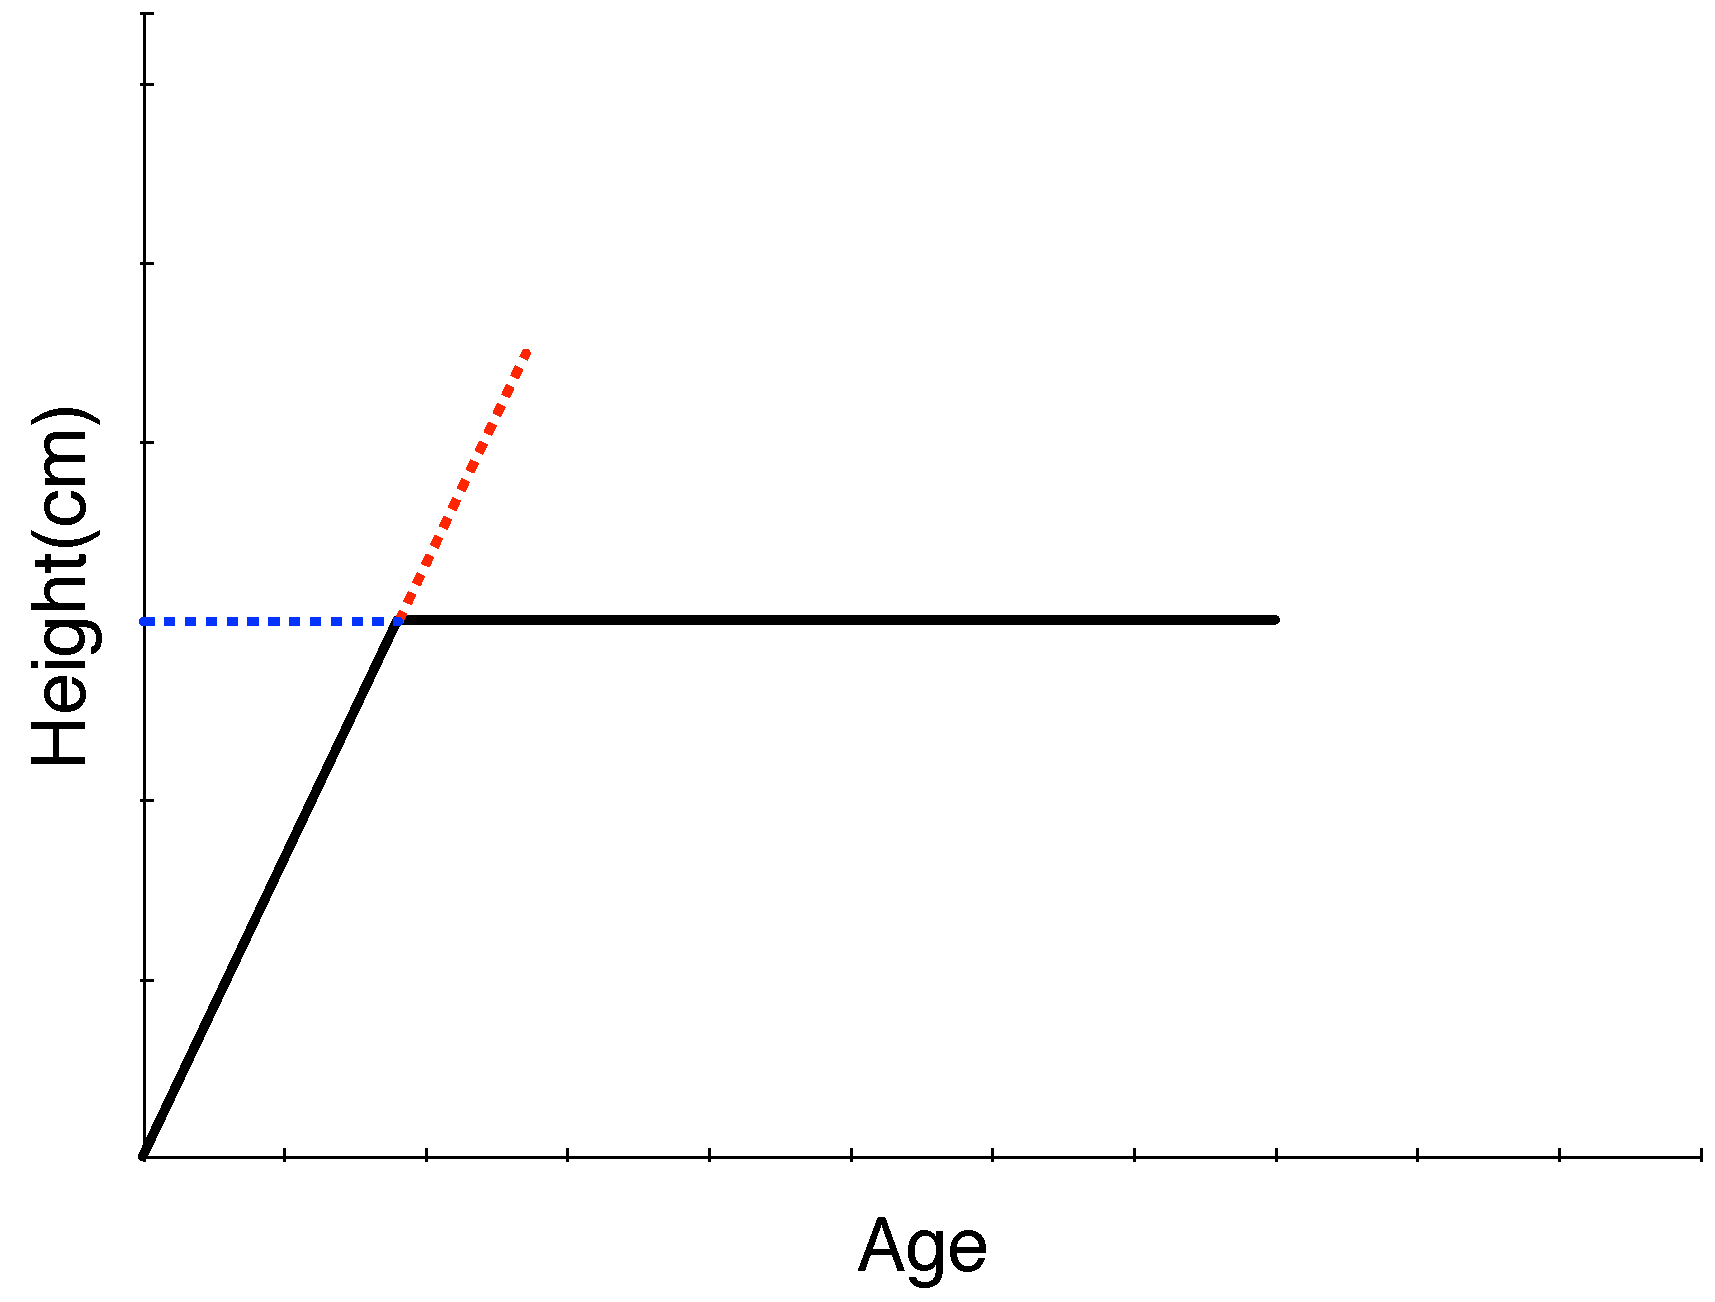
\includegraphics[width=1\textwidth]{lectMM/ageVsHeightV1.pdf}
\end{column}
\end{columns}
\end{frame}
%***********************************************************

\begin{frame}{Mixture of Experts Summary}

\begin{itemize}
\item Used for regression/classification
\begin{itemize}
	\item In ``classical'' GLMs
	\item Use dot product $x \cdot r = \sum_j x_j \times r_j$ to get ``natural'' parameter for error distribution
	\item Ex: Normal (least squares) regression:
	$$f (y | x) = \textrm{Normal} (y | x \cdot r, \sigma^2)$$
\end{itemize}
\item Now, let's have a mixture of these
\begin{itemize}
	\item Instead of $r$, we have $r_1, r_2, ..., r_k$
	\item Instead of $\sigma^2$, we have $\sigma^2_1, \sigma^2_2, ..., \sigma^2_k$
\end{itemize}
\item And then we use a ``softmax gating network'' to get $\pi$... that is:
	$$\pi_j = \frac{\exp (x \cdot \eta_j)}{\sum_{j'} \exp (x \cdot \eta_{j'})}$$
\end{itemize}
\end{frame}
%***********************************************************

\begin{frame}{Mixture of Experts Summary}

\begin{itemize}
\item So PDF is:
$$P(x_1, x_2, ..., x_n) = \prod_i \left( \sum_j \frac{\exp (x_i \cdot \eta_j)}{\sum_j' \exp (x_i \cdot \eta_{j'})}  \textrm{Normal} (x_i | x_i \cdot r_j, \sigma^2_j) \right)$$
\item $\eta_j$ is the set of gating coefficients for mixture $j$
\item The denominator normalizes the values, so we have probabilities
\item Basically, we are using a softmax function to decide the mixture
\item $\pi$ was a vector before
\item Now, $\pi$ is a vector whose value is dependent on the vector of $x$s
\item If we have a large dot product value it's highly likely that the $y$ value (output) will be generated by the $j$th component
\item Smaller ages are to the left, larger are to the right
\end{itemize}

\end{frame}
%***********************************************************

\begin{frame}{General Question: How to Choose Mixture Size}

\begin{itemize}
\item In last example...
\begin{itemize}
\item With four mixture components, could have two growth trends (women and men)
\item So probably, four is better than two here
\end{itemize}
\item How to choose in general case?
\begin{itemize}
\item Guess!  Then see if it is useful
\end{itemize}
\item Not good enough?  Are some alternatives
\begin{itemize}
\item Information theoretic methods (choose model that is able to encode data most efficiently)
\item Bayesian methods (put a prior on the number of components... ``infinite mixture models'')
\end{itemize}
\end{itemize}
	
\end{frame}
%***********************************************************
\begin{frame}{Questions?}
\begin{itemize}
	\item What do we know now that we didn't know before?
\begin{itemize}
	\item We understand that data can be generated by /represented as a mixture of different distributions
	\item We know about a Dirichlet distribution that can generate probability vectors
\end{itemize}

	\item How can we use what we learned today?
\begin{itemize}
	\item We can better model complex data by using mixture models
	\item We can combine simpler models into more complex models to get better predictions
\end{itemize}
\end{itemize}
\end{frame}


\end{document}
